\artigotrue
\chapter{MODELO CONCEITUAL DE PEDOGÊNESE DA BACIA DO DNOS}
\chapternote{Colaboraram na preparação deste manuscrito: Pablo Miguel (UFPel), Jean Michel Moura Bueno (UFSM), 
Ricardo Simão Diniz Dalmolin (UFSM), Andrisa Balbinot (UFSM), Lúcia Helena Cunha dos Anjos (UFRRJ), Gustavo de 
Mattos Vasques (Embrapa Solos), e Gerard B. M. Heuvelink (ISRIC -- World Soil Information).}
\shorttitle{Modelo Conceitual de Pedogênese}
\label{chap:chap03}
%\SweaveUTF8


\def\ptkeys{Província Geológica do Paraná. Bacia do DNOS. Rebordo do Planalto. Fatores de formação do solo. 
Pedogênese}

\begin{chapterabstract}{brazilian}{\ptkeys}
O presente manuscrito apresenta o modelo conceitual de pedogênese -- uma descrição explícita dos fatores e 
processos de formação do solo que determinam as características do solo e o seu padrão de distribuição 
espaço-temporal -- da bacia de captação do reservatório do Departamento Nacional de Obras de 
Saneamento-Companhia Riograndense de Saneamento (DNOS-CORSAN), localizada no sul do Brasil. O clima é 
subtropical úmido sem estação seca definida. O relevo é plano a montanhoso (variação de altitude entre 139 e 
\SI{475}{\m} acima do nível do mar), com vales encaixados que influenciam a precipitação e o fluxo radiativo 
nas diferentes superfícies geomórficas. A geologia é constituída pela sequência de três formações: rochas 
sedimentares (arenito fluvial), seguidas de rochas ígneas (basaltos-andesitos toleíticos e vitrófilos, 
riólitos-riodacitos granofíricos) intercaladas por rochas sedimentares (arenito eólico). Depósitos do 
Quaternário aparecem nas partes mais baixas. A geomorfologia atual é resultado dos processos erosivos do 
Terciário e Quaternário. A dissecação atual é fraca devido ao clima que favorece a instalação e permanência de 
vegetação exuberante. Três unidades morfoestruturais são identificadas: no topo, o Planalto, com relevo 
suave-ondulado a ondulado, seguido pelo Rebordo do Planalto, com ampla variação altimétrica, declividade 
acentuada e escarpas abruptas; na base, a Depressão Periférica, com formas agradacionais de planície fluvial. 
Nas partes altas, a rede de drenagem apresenta padrão bem definido, geralmente retangular, determinada pelas 
falhas e/ou fraturas. Já nas áreas mais baixas, devido aos processos de deposição sedimentar e erosão fluvial, 
sua configuração é sinuosa. Ali encontram-se um lençol freático próximo da superfície do solo e cursos de água 
perenes. O uso da terra para produção agrossilvopastoril foi intenso em tempos pretéritos e resultou em forte 
degradação do solo. O abandono de muitas áreas degradadas permitiu a regeneração da vegetação natural, 
resultando na atual ocupação com florestas e vegetação secundária de \SI{\pm60}{\percent}. Em geral, o solo é 
pouco profundo devido ao predomínio de condições de forte declividade. É comum encontrar solo raso mesmo em 
áreas de maior estabilidade como fruto da degradação pelo uso agrícola. O solo é mais profundo no Planalto, nos 
terraços do Rebordo, nas coxilhas (colinas) de relevo suave-ondulado a ondulado, e nas planícies aluviais. A 
textura é mais fina e homogênea ao longo do perfil quando desenvolvido a partir de rochas ígneas. As 
características do solo nas planícies aluviais são determinadas pela presença constante de lençol freático 
próximo da superfície.
\end{chapterabstract}

\def\enkeys{Paraná Geological Province. DNOS Catchment. Plateau Border. Soil-forming factors. Pedogenesis}
  
\begin{chapterabstract}{english}{\enkeys}
This document presents the conceptual model of pedogenesis -- an explicit description of soil-forming factors 
and processes that determine the spatio-temporal distribution of soil properties  -- of the catchment of the 
reservoir of the Departamento Nacional de Obras de Saneamento-Companhia Riograndense de Saneamento 
(DNOS-CORSAN), located in southern Brazil. Climate is subtropical humid without a dry season. Relief varies 
between plain and mountainous, with enclosed valleys (elevation ranging between \num{139} and \SI{475}{\m} 
above sea level) that determine rainfall volume and radiative flux on different surfaces. The geology is 
composed of a sequence of three formations: consolidated sedimentary rocks (fluvial sandstone), followed by 
basic and acid igneous rocks (andesite-basalt and rhyolite-rhyodacite), interlayered with consolidated 
sedimentary rocks (aeolian sandstone). Unconsolidated Quaternary colluvial deposits occur in the lower 
portions of the landscape. Current geomorphology is a result of erosive processes of the Tertiary and 
Quaternary. Landscape dissection is weak due to the current climate that favours the installation and 
maintenance of an exuberant vegetation. There are three morphostructural units: at the top, the 
\textit{Planalto} (Plateau), with gently-rolling to sloping relief, followed by the \textit{Rebordo do 
Planalto} (Plateau Border), with wide altimetric variation, steep slopes and abrupt cliffs; at the bottom, 
the \textit{Depressão Periférica} (Peripheral Depression), composed of aggradational fluvial plains. In 
higher altitudes, the drainage network has a well defined pattern, generally rectangular, determined by the 
faults and/or fractures. In the lower areas, its configuration is sinuous due to sediment deposition and 
fluvial erosion, with the presence of water table close to the surface and perennial water streams. Land use 
for agrosilvopastoral production was intense in past times, resulting in severe soil degradation. Recent 
abandonment of many degraded areas allowed the regeneration of natural vegetation, resulting in 
\SI{\pm60}{\percent} of the area being now occupied with forest and secondary vegetation. The soil is 
predominantly shallow due to the dominance of steep slopes. Even in gently-sloping terrain it is common to 
find shallow soils as a result of soil degradation. Deeper soil can be found in the Planalto, in the terraces 
of the Rebordo, and in the small hills with gently-rolling slopes and alluvial plains. Soil texture is finer 
and more homogeneous throughout the soil profile in soil developed from igneous rocks. Soil features in the 
alluvial plains are determined by the constant presence of the water table close to the surface.
\end{chapterabstract}

\formatchapter

\section{APRESENTAÇÃO}
\label{sec:chap03-apresentacao}

A modelagem espacial do solo inicia com a definição de um \emph{modelo conceitual de pedogênese}. Um modelo 
conceitual de pedogênese constitui uma representação verbal da realidade sob estudo que inclui a descrição 
explícita dos fatores e processos de formação do solo que determinam as características do solo e o seu padrão 
de distribuição espaço-temporal. Isso requer a reunião de toda a informação ambiental disponível e aplicação 
dos conceitos de relação solo-paisagem, desenvolvimento do solo em catenas, ou outro modelo teórico de 
explicação da variação espacial do solo.

O presente manuscrito apresenta o modelo conceitual de pedogênese da bacia de captação do reservatório do 
Departamento Nacional de Obras de Saneamento-Companhia Riograndense de Saneamento (DNOS-CORSAN), localizada 
na divisa entre os municípios de \itaara{} (ao norte) e \santamaria{} (ao sul), na porção sul da 
\baciaparana{}, estado do Rio Grande do Sul, Brasil (\autoref{fig:chap03-location}). A bacia de captação do 
reservatório do DNOS-CORSAN corresponde à cabeceira da bacia hidrográfica do \riovacacaimirim{}, tributário do 
\riojacui{} e, consequentemente, do \rioguaiba{} e da \lagoadospatos{}. A bacia de captação do reservatório do 
DNOS-CORSAN cobre uma área de \SI{\pm29}{\square\kilo\metre} e alimenta um reservatório com volume máximo de 
\SI{\pm3800000}{\cubic\metre} em uma área inundada de \SI{0,74}{\square\kilo\metre}. Este reservatório 
contribui com até \SI{30}{\percent} do abastecimento de água da cidade de Santa Maria \cite{Dias2003, 
DillEtAl2004, Miguel2010}.

\begin{figure}[!ht]
\centering
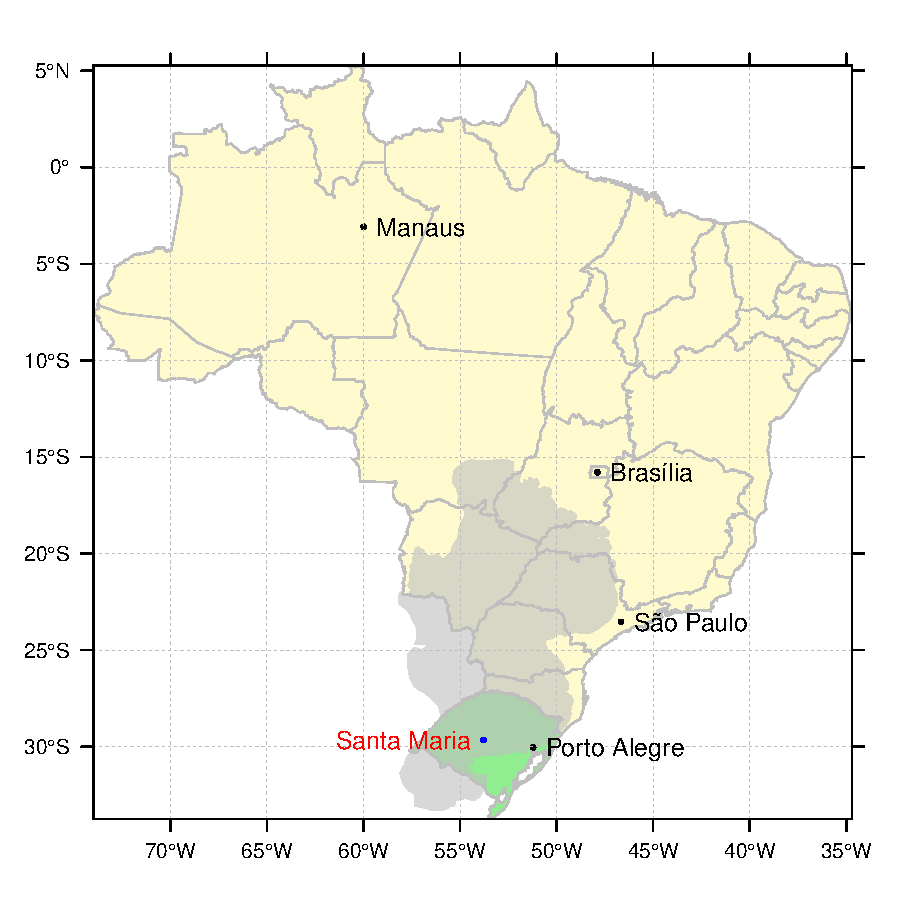
\includegraphics[width=0.90\textwidth]{fig/chap03-location}
\caption[Localização da bacia de captação do reservatório do DNOS-CORSAN, em Santa Maria, RS, 
Brasil]{Localização da bacia de captação do reservatório do Departamento Nacional de Obras de 
Saneamento-Companhia Riograndense de Saneamento no Município de Santa Maria (em azul), Estado do Rio 
Grande do Sul (em verde), Brasil, na porção sul da Província Geológica do Paraná (em cinza).}
\label{fig:chap03-location}
\end{figure}

\def\footsolosdors{\footnote{O grupo está registado no Diretório dos Grupos de Pesquisa no Brasil 
(\href{http://dgp.cnpq.br/dgp/espelhogrupo/9373361709890764}{DGP}) mantido pelo CNPq.}}

Os estudos em modelagem espacial do solo na bacia do DNOS -- abreviatura de bacia de captação do reservatório 
do DNOS-CORSAN -- iniciaram no ano de \num{2008} com o grupo de pesquisa \emph{Gênese, composição e 
comportamento dos solos do RS}\footsolosdors{}, sediado no Departamento de Solos da Universidade Federal de 
Santa Maria (\ufsm). Devido à limitação de recursos, o grupo de pesquisa optou por restringir seus estudos em 
modelagem espacial do solo à uma parte da bacia do DNOS. A área escolhida cobre \SI{\pm60}{\percent} de toda a 
bacia do DNOS, o que corresponde à uma área de \SI{\pm18}{\square\kilo\metre}. A área de estudo foi escolhida 
por apresentar acesso facilitado, além de englobar as principais formações geológicas, geoformas, usos da 
terra, e vegetação presentes na bacia do DNOS (\autoref{fig:chap03-perspective}).

\begin{figure}[!ht]
\centering
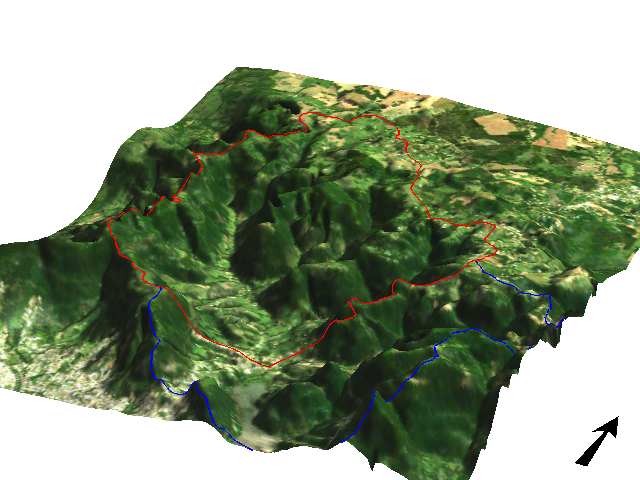
\includegraphics[width = 0.90\textwidth]{fig/chap03-perspective}
\caption[Localização da área de estudo na bacia do DNOS.]{Localização da área de estudo (em vermelho) na 
bacia de captação do reservatório do Departamento Nacional de Obras de Saneamento-Companhia Riograndense de 
Saneamento (DNOS-CORSAN) (em azul). A área de estudo, cujo relevo é bastante acidentado e o uso da terra 
predominante é floresta natural, possui aproximadamente \SI{4}{\km} de largura e \SI{5}{\km} de comprimento, 
o que corresponde a \SI{\pm60}{\percent} da área bacia do DNOS-CORSAN.}
\label{fig:chap03-perspective}
\end{figure}

\section{CLIMA}
\label{sec:chap03-clima}

% Footnote %%%%%
\def\footcfa{\footnote{Mais informações sobre o tipo climático Cfa podem ser encontrados na 
\href{https://pt.wikipedia.org/wiki/Clima_subtropical_\%C3\%BAmido}{Wikipedia}.}}

O clima local é classificado como Cfa\footcfa{} -- subtropical úmido sem estação seca definida --, com 
temperatura média anual de \SI{19,1}{\celsius}. As temperaturas podem alcançar \SI{>40}{\celsius}, no verão, e 
valores negativos no inverno \cite{HeldweinEtAl2009}. A precipitação média anual é de \SI{1708}{\milli\metre} 
bem distribuídos ao longo do ano \cite{Maluf2000}. Predominam os ventos (em ordem de frequência) do quadrante 
leste (frio, úmido e de intensidade fraca a moderada), oeste (frio, seco e de intensidade fraca a moderada) e 
norte (quente, seco e de intensidade moderada a forte) \cite{HeldweinEtAl2009}.

O padrão predominante das chuvas é o avançado, caracterizado por ter seu pico de maior intensidade no início 
da precipitação \cite{MehlEtAl2001}. As chuvas de maior intensidade ocorrem nos meses do final da primavera, 
verão e início do outono \cite{MouraBueno2012}. Como resultado desse padrão, as chuvas de inverno são as 
menos erosivas, mesmo que o conteúdo de água do solo permaneça elevado durante todo o período. O padrão de 
precipitação também é condicionado pelo relevo. Observações feitas em três locais durante o ano de \num{2011}, 
marcado por forte estiagem, mostram variação na lâmina total precipitada entre \num{1317} e \SI{1411}{\mm} 
\cite{MouraBueno2012}. Assim, o relevo plano a montanhoso, com vales encaixados, parece condicionar a formação 
de diferentes regiões microclimáticas, refletindo no volume e intensidade das chuvas \cite{MouraBueno2012}.

O relevo também deve condicionar o fluxo radiativo que atinge as diferentes superfícies. Apesar de não haver 
estudos que demonstrem a efetividade desse fenômeno na área, é reconhecido que grande parte da superfície em 
terrenos de topografia complexa é influenciada pelo efeito de sombreamento, sobretudo nas primeiras horas da 
manhã e no final da tarde \cite{OliphantEtAl2003}. Além disso, a declividade do terreno possui forte 
influência sobre o ângulo de interceptação da radiação solar pelas superfícies \cite{Birkeland1999}. Como 
consequência, deve ocorrer variações na temperatura e conteúdo de água no solo nas diferentes superfícies. Os 
meses de inverno são marcados por ainda menor disponibilidade de radiação solar devido à alta frequência de 
nevoeiros, sobretudo nas partes mais baixas, com valores normais de insolação de \SI{5,1}{\hour\per\day} 
\cite{HeldweinEtAl2009}. Além disso, devido à variação de altitude entre \num{139} e \SI{475}{\metre}, deve 
ocorrer diferença na temperatura da ordem de \SI{4}{\celsius} entre a parte mais baixa e a parte mais alta 
\cite{HeldweinEtAl2009}.

\section{GEOLOGIA}
\label{sec:chap03-geologia}

A geologia é bastante complexa, sendo constituída de três formações geológicas, além de depósitos coluviais 
e aluviais do Quaternário. A literatura sobre o tema é vasta \cite{Bortoluzzi1974, Brasil1980, 
GasparettoEtAl1988, MacielFilho1990, Machado1998, PieriniEtAl2002, MarquesEtAl2005, Milani2005, Pinto2005, 
CPRM2007, Pedron2007, Sartori2009, NascimentoEtAl2010, WerlangEtAl2010, PedronEtAl2012}, e uma revisão da 
mesma é apresentada aqui.

% Link %%%%%
\def\caturrita{\href{https://pt.wikipedia.org/wiki/Forma\%C3\%A7\%C3\%A3o_Caturrita}{Formação Caturrita}}

Na base da sequência estratigráfica, em elevações abaixo de \SI{\pm200}{\metre}, está a \caturrita{}, 
constituída de material sedimentar depositado em ambiente fluvial no Triássico Superior. Sua composição é 
diversa, apresentando seixos de siltito argiloso vermelho na base, seguido de arenito avermelhado de 
granulometria fina à média, composição quartzosa e matriz argilosa, podendo ainda conter considerável teor de 
feldspato, sobreposto por siltito e folhelho também avermelhados. Em geral, a granulometria do arenito é mais 
grosseira e menos argilosa na base da deposição. Devido à sua origem fluvial, a Formação Caturrita apresenta 
marcada estratificação cruzada acanalada e tabular. A origem fluvial também resulta em significativa variação 
espacial na granulometria do arenito, identificada pelo contraste entre áreas de maior cimentação e coesão, 
com outras de maior condutividade hidráulica. Imediatamente acima da Formação Caturrita encontra-se, ora a 
Formação Botucatu, ora a Sequência Inferior da Formação Serra Geral.

% Link %%%%%
\def\serrageral{\href{http://pt.wikipedia.org/wiki/Forma\%C3\%A7\%C3\%A3o_Serra_Geral}{Formação Serra Geral}}

Em elevações entre \num{\pm200} e \SI{\pm350}{\metre} está a Sequência Inferior da \serrageral{} 
(basaltos-andesitos toleíticos). As rochas básicas são de coloração cinza-escura e são constituídas de 
plagioclásio cálcico, clinopiroxênio, magnetita e material intersticial de quartzo e material desvitrificado. 
Em elevações superiores a \SI{\pm350}{\metre} está a Sequência Superior da Formação Serra Geral (vitrófilos, 
riólitos-riodacitos granofíricos). As rochas ácidas apresentam cor cinza-clara, estrutura microcristalina e 
são constituídas de cristais e plagioclásio, clinopiroxênios, hornblenda uralítica e magnetita. A origem 
desse material remonta o Cretáceo, quando sucessivos derrames de lavas de origem vulcânica fissural ocorreram 
durante aproximadamente \num{10} milhões de anos em toda a Bacia do Paraná. Esses eventos ocorreram ao mesmo 
tempo em que iniciava-se a separação das plataformas continentais que hoje constituem a América do Sul e 
África, marcando o final da existência do supercontinente Pangeia.

% Link %%%%%
\def\botucatu{\href{http://pt.wikipedia.org/wiki/Forma\%C3\%A7\%C3\%A3o_Botucatu}{Formação Botucatu}}

O arenito eólico constituinte da \botucatu{} é encontrado tanto assentado sobre a Formação Caturrita, como no 
interior da Formação Serra Geral (arenito \emph{intertrap}). Trata-se de arenito quartzoso de granulometria 
fina à média, contendo feldspato alterado e cimentado por sílica ou por óxido de ferro, que lhe confere a 
coloração rosa-avermelhada. Sua deposição teve início no Cretáceo Inferior, período em que a Bacia do Paraná 
estava sob influência de clima desértico. Essa condição climática continuou durante todo o período em que 
ocorreram as dezenas de eventos de vulcanismo fissural, fazendo com que os mesmos fossem sucedidos por 
deposições eólicas de duração variável. Como a duração e a quantidade de material depositado pelos eventos de 
vulcanismo fissural era variável, assim como o intervalo de tempo entre cada novo evento e a intensidade das 
deposições de sedimentos eólicos, a espessura das camadas do arenito eólico e das rochas vulcânicas é bastante 
variável. Além disso, devido aos diversos eventos de subsidência que ocorreram no eixo central da Bacia do 
Paraná, com consequente soerguimento de suas bordas, as camadas dessas rochas possuem diferentes inclinações 
ao longo de sua faixa de exposição, sendo caracteristicamente ondulada e com suave tendência de inclinação 
para sudoeste.

As deposições do Quaternário são constituídas por depósitos coluviais e aluviais. Em elevações entre 
\num{\pm200} e \SI{\pm300}{\metre} encontram-se depósitos coluviais de material proveniente de uma ou ambas as 
Formações Serra Geral (fragmentos de tamanho variado) e Botucatu. Em elevações abaixo de \SI{\pm200}{\metre} 
são mais comuns os depósitos coluviais de uma ou ambas as Formações Botucatu e Caturrita. Esses depósitos 
ocorrem de maneira descontínua nas encostas. Próximo aos cursos de água na porção mais baixa da bacia e no 
entorno do reservatório, encontram-se depósitos fluviais recentes, geralmente constituídos de fragmentos 
arredondados (seixos) de tamanho variável e/ou sedimentos arenosos. Em pequenas áreas abaciadas e mal 
drenadas, os sedimentos apresentam granulometria mais fina.

\section{GEOMORFOLOGIA}
\label{sec:chap03-geomorfologia}

A área de estudo está situada na porção sul da Bacia Sedimentar do Paraná. Assim, as geoformas atuais são 
resultado dos processos erosivos que ocorreram durante o Terciário e o Quaternário \cite{Sartori2009}, após as 
últimas deposições de lavas vulcânicas e de sedimentos eólicos. Durante esse período, a esculturação da 
paisagem foi determinada pelas alternações entre climas úmidos, semiáridos e áridos \cite{Sartori2009}. 
Atualmente, o clima subtropical úmido favorece a instalação e permanência de vegetação mais eficiente na 
redução do processo de dissecação da paisagem \cite{Sartori2009, NascimentoEtAl2010}. Isso permite que as 
superfícies geomórficas atinjam maior estabilidade e maturidade, embora o uso agrícola das terras tenha 
acelerado, pontualmente, os processos erosivos na área devido à limitada adoção de práticas conservacionistas 
(\autoref{sec:chap03-landuse}).

A bacia do DNOS é abrangida pela unidade morfoestrutural do Rebordo do Planalto da Bacia do Paraná 
\cite{NascimentoEtAl2010}. O Rebordo do Planalto é caracterizado pela ampla variação altimétrica, declividade 
acentuada e escarpas abruptas, apresentando formas denudacionais com topos convexos (fluxo hídrico 
divergente), aguçados e em formas de escarpas. Nesses locais, as vertentes assumem forma retilínea com grande 
desnível \cite{NascimentoEtAl2010}, muitas vezes interrompidas por degraus ou patamares, na maioria das vezes 
encaixadas em falhas e/ou fraturas. Esses patamares são resultado da ação diferencial dos processos 
denudacionais sobre a paisagem, geralmente condicionados pela resistência do material de origem, seja ela 
química/mineralógica (rochas vulcânicas básicas vs. ácidas), física/granulométrica (rochas vulcânicas versus 
sedimentares), ou estrutural (padrão de diaclasamento vertical vs. horizontal das rochas vulcânicas) 
\cite{Holtz2003, Pedron2007, StreckEtAl2008}. Entretanto, em algumas situações, os patamares são formados por 
depósitos coluviais -- mesmo nas partes altas do Rebordo do Planalto -- resultantes de movimentos de massa 
causados por eventos pluviométricos de elevada intensidade e/ou duração \cite{PinheiroEtAl2004, 
PaisaniEtAl2010}. Nesses casos, os patamares possuem menor dimensão e maior declividade. Em outras situações, 
os patamares coluviais, sobretudo aqueles originados dos arenitos da Formação Botucatu, formam 
vertentes alongadas e com menor inclinação, que chegam até a margem dos cursos de água.

Como a bacia do DNOS se encontra em uma região de transição morfoestrutural, as características 
geomorfológicas das porções mais altas e mais baixas da paisagem são similares àquelas encontradas nas 
unidades morfoestruturais adjacentes, respectivamente, o Planalto e a Depressão Periférica. O Planalto é 
marcado pelo relevo suave-ondulado a ondulado, com formas denudacionais de superfícies planas com topos 
convexos (fluxo hídrico divergente). Nesses locais, as vertentes assumem forma convexa levemente ondulada, 
muitas vezes encaixadas em falhas e/ou fraturas \cite{NascimentoEtAl2010}. Já a Depressão Periférica é marcada 
pelo acúmulo de sedimentos provenientes do Planalto e do Rebordo do Planalto, formando planícies aluviais que 
se intercalam entre as coxilhas (denominação regional de colinas). Ali predominam as formas agradacionais de 
planície fluvial e formas denudacionais com topos convexos e superfícies planas. As últimas correspondem às 
coxilhas de algumas dezenas de metros de altitude, geralmente formadas sobre o substrato da Formação Caturrita 
e assentadas na base do Rebordo do Planalto \cite{GasparettoEtAl1988}. Essas coxilhas constituem divisores de 
água de pequena amplitude comumente usados na subdivisão da bacia do DNOS em pequenas sub-bacias 
\cite{Marins2004, Sartori2009}. Nesses locais as vertentes costumam ser alongadas e assumem a forma 
predominantemente côncava devido aos processos de deposição sedimentar e erosão fluvial, muito fracos sob a 
atual condição climática \cite{NascimentoEtAl2010, WerlangEtAl2010}.

A grande heterogeneidade geomorfológica da bacia do DNOS se traduz em uma grande heterogeneidade textural 
do relevo, ou rugosidade, resultante da ação climática ao longo do tempo geológico \cite{NascimentoEtAl2010}. 
Entretanto, em menor escala, a ação antrópica também atuou sobre a configuração geomorfológica da área 
(\autoref{sec:chap03-landuse}). O principal efeito se deu pela erosão da camada superficial do solo, cultivado 
intensivamente sem adoção de práticas conservacionistas ao longo de inúmeras décadas \cite{Menezes2008, 
Sturmer2008, Miguel2010, SamuelRosaEtAl2011a}. Além disso, a abertura de caminhos para acesso às áreas de 
produção nos patamares do Rebordo do Planalto e nos topos de morros proporcionou a formação de canais de 
concentração e escoamento dos fluxos hídricos superficiais, levando à formação inicial de voçorocas. Obras de 
maior expressividade, como ferrovias, ruas e rodovias pavimentadas, conjuntos habitacionais e construções 
isoladas, as quais envolvem operações de terraplanagem e aterramento, também resultaram em modificações 
localizadas na geomorfologia da área. Por fim, a construção do reservatório possibilitou a formação de uma 
área de agradação da paisagem bastante estável em seu entorno, uma vez que o sedimento removido do Planalto e 
do Rebordo do Planalto já não são mais transportados a jusante.

\section{HIDROGRAFIA}
\label{sec:chap03-hidrografia}

A hidrografia da área é condicionada pelas condições geomorfológicas, geológicas, pedológicas e climáticas, ao 
mesmo tempo em que exerce forte influência sobre a modelagem da paisagem \cite{NascimentoEtAl2010}. Como a 
bacia do DNOS é abrangida pela unidade morfoestrutural do Rebordo do Planalto da Bacia do Paraná 
(\autoref{sec:chap03-geomorfologia}), a drenagem apresenta padrão bem definido, geralmente retangular, 
determinado pelas falhas e/ou fraturas \cite{Bortoluzzi1974, GasparettoEtAl1988, NascimentoEtAl2010}. A 
própria formação da bacia do DNOS se deve a existência de falhas e/ou fraturas \cite{GasparettoEtAl1988}. A 
principal e maior delas localiza-se no eixo central da bacia, onde atualmente está localizado o leito do Rio 
Vacacaí-Mirim. Quanto aos tributários do Rio Vacacaí-Mirim, a maioria possui leito assentado sobre outras 
falhas e/ou fraturas de menor dimensão perpendiculares àquela do eixo central da bacia.

Nas áreas mais baixas, cujas características geomorfológicas se assemelham à Depressão Periférica, a drenagem 
apresenta configuração sinuosa, resultado dos processos de deposição sedimentar e erosão fluvial 
\cite{PaivaEtAl2001, SutiliEtAl2009}. Como o relevo é plano a suave-ondulado, e as vertentes longas e 
predominantemente côncavas, o lençol freático fica próximo da superfície do solo. A variação das condições 
meteorológicas ao longo do ano fazem com que o lençol freático apresente flutuação significativa, mantendo o 
conteúdo de água do solo elevado durante os meses mais frios (menor evapotranspiração) 
\cite{HeldweinEtAl2009}. Isso também favorece a ocorrência de inundações, sobretudo nas proximidades dos 
cursos de água e do reservatório \cite{Goldani2006}.

Muitos cursos de água localizados na áreas cujas características geomorfológicas se assemelham ao Planalto, 
assim como no Rebordo do Planalto e nas coxilhas assentadas em sua base, são sazonais. Em geral, esses cursos 
de água estão em atividade apenas nos meses mais frios do ano, quando a disponibilidade de água no ambiente é 
maior, ou durante os eventos de precipitação de forte intensidade, que ocorrem nos meses de verão 
\cite{HeldweinEtAl2009, MouraBueno2012}. Os cursos de água do Rebordo do Planalto costumam apresentar leito 
raso e pedregoso, muitas vezes assentado sobre rochas da Formação Serra Geral \cite{SutiliEtAl2009}. Já os 
cursos de água localizados nos patamares e coxilhas costumam ser rasos, se assentados sobre rochas da Formação 
Caturrita, ou profundos, se assentados sobre rochas da Formação Botucatu ou depósitos coluviais, formando 
voçorocas. Segundo relatos de alguns dos moradores mais antigos da bacia do DNOS, muitas nascentes e pequenos 
cursos de água já perderam totalmente sua atividade, sobretudo quando localizadas no interior ou à jusante de 
áreas de uso antrópico intensivo.

Dado que a declividade e o desnível entre a parte mais baixa e a parte mais alta da área são acentuados, as 
cheias costumam apresentar velocidade e vazão bastante grandes \cite{PaivaEtAl2001, SutiliEtAl2009}. Em média, 
nos \SI{7}{\km} de extensão do Rio Vacacaí-Mirim, da nascente até o reservatório, a declividade média é de 
\SI{0,03}{\m\per\m}. Isso representa um desnível de \SI{\pm210}{\m}, o que resulta em um tempo de concentração 
da bacia estimado de \SI{3}{\hour} \cite{PaivaEtAl2001}. Essas características causam erosão severa nas 
margens dos cursos de água nas áreas mais baixas (depósitos aluviais), sobretudo nos raios externos das 
curvas, onde a velocidade da água é maior \cite{SutiliEtAl2009}. Em alguns trechos, os cursos de água chegaram 
a ter sua largura duplicada em menos de uma década, resultando no aumento da sinuosidade e do nível de fundo 
\cite{PaivaEtAl2001}. Esses eventos comprometem áreas de produção agrícola, bem como a estrutura de 
residências e vias públicas localizadas nas margens dos cursos de água. Grande parte do material removido das 
margens dos cursos de água é transportado para dentro do reservatório, que já perdeu mais de 
um terço de sua capacidade inicial de armazenamento de água \cite{DillEtAl2004}.

\section{USO DA TERRA E VEGETAÇÃO}
\label{sec:chap03-landuse}

A bacia do DNOS foi intensamente ocupada em tempos pretéritos para produção agrossilvopastoril de pequeno 
porte (agricultura familiar) usando sistemas de cultivo convencional com aração periódica e queimada. A grande 
quantidade, extensão e boa distribuição da rede viária em toda a área é uma forte evidência dessa ocupação. A 
área também é cortada por uma estrada férrea e avizinha uma rodovia federal, ambas muito movimentadas. 
Entretanto, nas últimas décadas, muitos caminhos internos das propriedades rurais foram desativados, fruto do 
abandono de muitas áreas de produção agrossilvopastoril, a maioria delas localizada nos topos dos morros, 
patamares do Rebordo ou no fundo de vales, onde a manutenção dos caminhos é muito onerosa, especialmente 
quando distantes da sede das propriedades (\autoref{fig:chap05-land-use} e \autoref{fig:chap05-sat-image}). No 
passado, essas estradas internas possibilitavam o trânsito de pessoas e o transporte da produção 
agrossilvopastoril, a qual era usa para suprir as necessidades próprias, sendo o excedente comercializado às 
margens da estrada férrea e nas áreas urbanas do município. Atualmente, o tráfego existente está concentrado 
nas estradas principais e secundárias, enquanto alguns poucos caminhos internos ainda são utilizados para 
condução de rebanhos ou acesso a pequenas áreas de produção agrossilvopastoril. A maioria dos caminhos internos 
inativos está localizada no interior de áreas de floresta natural regenerada, o que dificulta a sua 
identificação com imagens aéreas ou orbitais. Em alguns casos, esses caminhos são utilizados em atividades de 
turismo, especialmente para caminhadas a pé, ou atividades esportivas com motocicletas (trilhas).

O abandono de muitas áreas de produção agrossilvopastoril possibilitou a regeneração da vegetação natural em 
grande parte da bacia do DNOS. Atualmente, a área ocupada por florestas e vegetação secundária (capoeira) 
representa \SI{\pm60}{\percent} da área total \cite{SamuelRosaEtAl2011a}. Isso mostra que, assim como toda a 
região do Rebordo do Planalto da Bacia do Paraná, o uso da terra para fins agrossilvopastoris na bacia do DNOS 
também foi desintensificado nas últimas décadas \cite{SEMA/UFSM2001, DillEtAl2004, Poelking2007, Miguel2010, 
SamuelRosaEtAl2011a, Dullius2012, TenCatenEtAl2012}. As áreas de floresta são encontradas nos mais diversos 
estádios de desenvolvimento, com os estratos intermediário e superior concentrando a maior parte dos 
indivíduos. As florestas originais, e secundárias em estádio avançado de desenvolvimento, são encontradas, 
predominantemente, em áreas de difícil acesso. Em geral, as áreas de floresta predominam nas regiões com maior 
declividade e solo raso e pedregoso. Tais condições pedológicas são resultado das condições geológicas e 
geomorfológicas e/ou da degradação causada pelo intenso uso da terra para produção agrossilvopastoril durante 
inúmeras décadas usando sistemas de cultivo convencional \cite{SamuelRosaEtAl2011a}.

A ocorrência de fragmentos florestais ao longo das margens dos cursos de água, estradas e próximo de 
edificações é comum. Nas formações mais jovens, é comum encontrar fragmentos de carvão e outros sinais do uso 
agrossilvopastoril num passado recente. As áreas sob vegetação secundária (capoeira) também ocorrem em toda a 
bacia do DNOS, predominantemente em locais de difícil acesso e acentuada declividade, geralmente interligados 
por caminhos internos, indicando sua utilização agrossilvopastoril no passado \cite{SamuelRosaEtAl2011a}. Sua 
composição florística varia entre as áreas, predominando espécies de porte herbáceo e arbustivo. O solo dessas 
áreas costuma ser menos pedregoso que nas áreas florestadas, mas apresentam profundidade semelhante 
\cite{SamuelRosaEtAl2011a}, possivelmente indicando que as atividades agrossilvopastoril foram encerradas 
antes do solo atingir seu nível máximo de degradação. Entretanto, a reserva de nutrientes do solo, assim como 
a sua fertilidade física, foram esgotadas a tal ponto que a vegetação secundária ainda não foi capaz de 
produzir melhorias significativas quando comparado com as condições originais \cite{Menezes2008, 
Zalamena2008}.

Apesar do abandono de muitas áreas de produção agrossilvopastoril nas últimas décadas, sobretudo aquelas com 
maior dificuldade de acesso, os caminhos internos utilizados para o escoamento da produção, mesmo depois de 
inativos, continuam associados ao processo de degradação do solo. Isso ocorre porque, na grande maioria dos 
casos, todo o fluxo da água de escoamento superficial proveniente dos eventos de precipitação é concentrado 
nesses caminhos internos, onde, geralmente, quantidade significativa de resíduos vegetais está depositada. 
Esse resíduo vegetal, mais a fração mineral do solo carregada pela enxurrada, costuma chegar com facilidade 
aos cursos de água. No caso dos caminhos internos ainda utilizados na condução de rebanhos bovinos, a produção 
de sedimentos minerais tende a ser ainda maior, haja vista o impacto mecânico do pisoteio animal sobre a 
desagregação do solo. Além disso, muitas áreas florestadas e sob vegetação secundária ainda são utilizadas 
para o pastoreio de bovinos e equinos \cite{SamuelRosaEtAl2011a}. Isso causa a degradação da camada 
superficial do solo, sobretudo pela sua compactação, dificultando a infiltração da água dos eventos de 
precipitação, o que resulta na perda da serapilheira \cite{ScheneiderEtAl1978}. Além disso, a própria 
regeneração natural é prejudicada, uma vez que plantas em estádio inicial de desenvolvimento e raízes 
superficiais são destruídas \cite{ScheneiderEtAl1978, HackEtAl2005}. O resultado desse processo é a redução da 
capacidade do solo em suportar o desenvolvimento potencial da floresta \cite{KonigEtAl2002}.

Dado que a bacia do DNOS também possui áreas com relevo plano a suave-ondulado e solo profundo, 
\SI{\pm30}{\percent} de sua superfície ainda é utilizada com atividades agrossilvopastoris ao longo de todo o 
ano, principalmente a pecuária bovina extensiva \cite{SamuelRosaEtAl2011a}. As áreas de produção animal 
extensiva predominam nas porções norte, sul e centro-oeste, ao longo dos cursos de água e estradas. O solo é 
mais profundo e menos pedregoso do que em áreas de floresta natural e vegetação secundária. É comum encontrar 
fragmentos de carvão e formações de microrrelevo devido ao uso de implementos agrícolas para o revolvimento do 
solo na maior parte desses locais, evidenciando seu uso agrícola num passado recente. Essas áreas podem ser 
divididas entre aquelas de campo sujo (pastagens naturais mal manejadas, com predomínio de vegetação de porte 
herbáceo-arbustivo) e campo limpo (pastagens naturais e perenes bem manejadas) \cite{SamuelRosaEtAl2011a}. Em 
geral, as áreas de campo sujo estão próximas a áreas de vegetação secundária (capoeira), com relevo mais 
declivoso e solo mais pedregoso e raso do que aquelas de campo limpo. Assim como nas áreas de floresta e sob 
vegetação secundária, a dinâmica de uso dessas áreas ao longo do tempo é bastante complexa, dificultando o 
estabelecimento de relações diretas com a maior parte das características do solo. Entretanto, sob o ponto de 
vista da reserva de nutrientes e matéria orgânica, o solo pode ser considerado pobre, uma vez que a exploração 
pecuária é totalmente extrativista e extensiva.

As atividades agrossilvopastoris que ocupam menor extensão territorial são a agricultura e a silvicultura. As 
áreas de lavoura anuais e bianuais estão dispersas em toda a área, geralmente localizadas em terrenos de 
menor declividade e solo medianamente profundo. Entretanto, algumas áreas de produção agrícola possuem 
declives superiores a \SI{50}{\percent} e solo raso e pedregoso \cite{SamuelRosaEtAl2011a}. Em qualquer das 
situações, as condições de degradação do solo costumam ser bastante avançadas devido ao emprego de sistemas 
convencionais de cultivo, exceto por algumas áreas de produção olerícola. As florestas plantadas 
(\textit{Eucalyptus spp.}) são implantadas em áreas com menor declividade e solo mais profundo, geralmente 
onde o acesso com máquinas é melhor, sobretudo pela necessidade de manejo e escoamento da produção. A área 
ocupada por essa atividade possui tendência de crescimento, haja vista os novos plantios existentes e o relato 
de alguns moradores \cite{SamuelRosaEtAl2011a}. Em geral, os novos plantios são implantados em áreas de 
produção agropecuária, seja pelo elevado nível de degradação do solo já atingido, seja pela redução da força 
de trabalho das famílias devido ao êxodo rural, ou pela maior lucratividade dessa atividade.

Por fim, as obras de engenharia e assentamentos urbanos são aquelas que ocupam a menor parte da bacia do DNOS. 
No que diz respeito à malha viária, a maior concentração ocorre na porção sul, junto ao maior assentamento 
urbano, localizado no entorno do reservatório. Entretanto, diversas construções são encontradas ao longo das 
estradas que cortam a área, muitas das quais são pertencentes a moradores do centro da cidade de Santa Maria e 
são utilizadas apenas como sítios de final de semana. O número de sítios de final de semana aumentou 
significativamente nas últimas décadas \cite{Goldani2006}, muitos dos quais construídos em locais 
inapropriados, como margens dos corpos de água e áreas com forte declividade. Esse processo de urbanização 
desordenada, que exigiu a realização de obras de corte e aterramento dos terrenos, é um importante 
contribuinte da carga de sedimentos recebida pelo reservatório anualmente, aos quais somam-se os resíduos 
domésticos e cloacais \cite{Goldani2006, PaivaEtAl2001, DillEtAl2004, MiguelEtAl2014}. Quanto às demais obras 
de engenharia, destacam-se os reservatórios de água, a maioria deles de pequena extensão, utilizados para a 
dessedentação animal. Como os cursos de água de maior volume estão localizados na porção sul da área, a maior 
parte dos reservatórios de água está na porção norte \cite{SamuelRosaEtAl2011a}. Além disso, a menor 
permeabilidade do solo e do substrato rochoso, bem como da condição topográfica, favorecem essa 
característica.

\section{PEDOLOGIA}

O solo da bacia do DNOS possui características com forte dependência do material de origem que, conforme 
descrito anteriormente, é um importante condicionante da geomorfologia e da hidrografia 
\cite{NascimentoEtAl2010}. Nas superfícies geomórficas mais estáveis, como no topo do Planalto (rochas 
vulcânicas), nos terraços do Rebordo (rochas vulcânicas e sedimentares) e nas coxilhas de relevo 
suave-ondulado a ondulado (rochas sedimentares), as condições ambientais são mais favoráveis ao 
desenvolvimento do solo em profundidade \cite{Moser1990}. O contrário ocorre nas áreas de relevo mais 
acidentado do Rebordo, onde acredita-se que a taxa de formação do solo seja semelhante à taxa de remoção 
natural \cite{Moser1990, DalmolinEtAl2006a, Sturmer2008, SamuelRosaEtAl2011a}. Além da condição 
geomorfológica, a resistência da rocha ao intemperismo também condiciona o desenvolvimento do solo em 
profundidade nesses locais \cite{Pedron2007}. Já nas planícies aluviais, as características do solo foram 
fortemente influenciadas pelo hidromorfismo e deposição sedimentar, geralmente resultando em solo de coloração 
acinzentada e maior profundidade do que nas área declivosas Rebordo \cite{Moser1990, Miguel2010}. A forte 
influência da geologia também aparece na textura do solo (\autoref{fig:chap03-clay-land-parent}). Enquanto os 
arenitos conferem textura arenosa ao solo, sobretudo aqueles da Formação Botucatu, as rochas vulcânicas 
conferem textura média ao solo, sobretudo os basaltos-andesitos toleíticos (\autoref{sec:chap05-geo-maps}).

\begin{figure}[!ht]
\centering
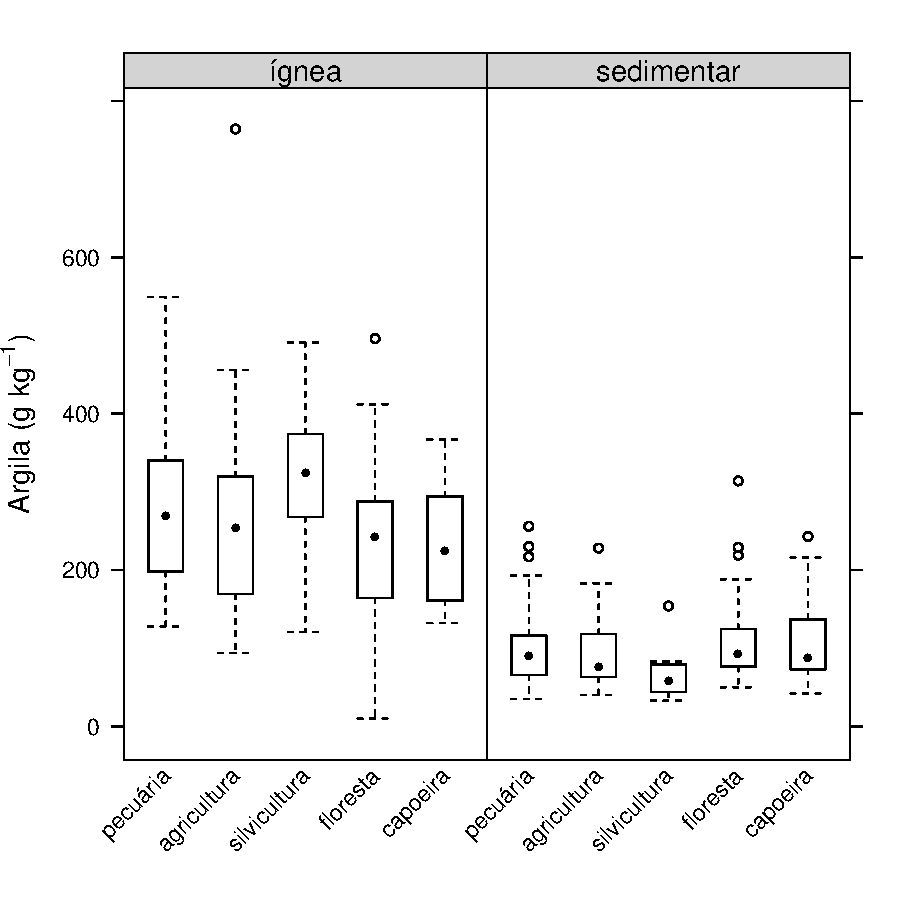
\includegraphics[width=0.60\textwidth]{fig/chap03-clay-land-parent}
\caption[Argila no solo e sua relação com o uso da terra e o material de origem do solo.]{
Distribuição do conteúdo de argila (\si{\gram\per\kilo\gram}) na camada superficial do solo (\SI{\leq20}{\cm}) 
e sua relação com o uso da terra e vegetação (pecuária, agricultura, silvicultura, floresta e capoeira) e o 
tipo de material de origem (ígnea -- rocha ígnea, ou sedimentar -- rocha sedimentar ou sedimentos diversos).
Solo desenvolvido a partir de material de origem sedimentar costuma apresentas conteúdo de argila inferior à 
solo desenvolvido a partir de material de origem ígnea. Em geral, essa relação é pouco influenciada pelo tipo 
de uso da terra. A exceção são as áreas destinadas à silvicultura localizadas no setor norte da bacia do DNOS, 
cujo solo desenvolveu a partir de material de origem ígnea. Ali a tendência é de o solo apresentar maior 
conteúdo de argila na camada superficial.}
\label{fig:chap03-clay-land-parent}
\end{figure}

Como a bacia do DNOS possui a maior parte de sua área em condições de declividade moderada à forte, e foi 
intensamente ocupada em tempos pretéritos para produção agrossilvopastoril com aração e queimada periódicas 
(\autoref{sec:chap03-landuse}), o solo é, predominantemente, pouco profundo. Nas áreas de declividade moderada 
à forte o solo costuma apresentar profundidade inferior à \SI{50}{\cm} até o contato lítico, sendo comum a 
ocorrência de pedregosidade e rochosidade abundantes \cite{Miguel2010}. Assim, predominam as classes 
taxonômicas Neossolo Litólico Distro-Úmbrico típico, Cambissolo Háplico Ta Eutrófico típico, Neossolo Litólico 
Eutro-Úmbrico típico e Neossolo Regolítico Distro-Úmbrico típico (\autoref{sec:chap05-soil-maps}). O efeito do 
uso inapropriado do solo para produção agrossilvopastoril aparece mesmo em algumas áreas de maior estabilidade
(topos de morros, patamares do Rebordo do Planalto e coxilhas) onde as condições para o desenvolvimento 
pedogenético são mais favoráveis \cite{Moser1990, MouraBueno2012}. Por exemplo, alguns patamares do Rebordo, 
inicialmente constituídos de colúvios sedimentares (arenito Botucatu) e vulcânicos (fragmentos de tamanhos 
variáveis), apresentam solo com superfície recoberta por fragmentos rochosos, fruto da forte erosão a que foi 
submetido, limitando a continuação de seu uso para atividades agrossilvopastoris \cite{MouraBueno2012}. Essas 
atividades também resultaram na depleção da fertilidade do solo, marcada atualmente pelos baixos conteúdo de 
carbono orgânico (\autoref{fig:chap03-orca-land-parent}) e capacidade de troca de cátions efetiva 
(\autoref{fig:chap03-ecec-land-parent}).

\begin{figure}[!ht]
\centering
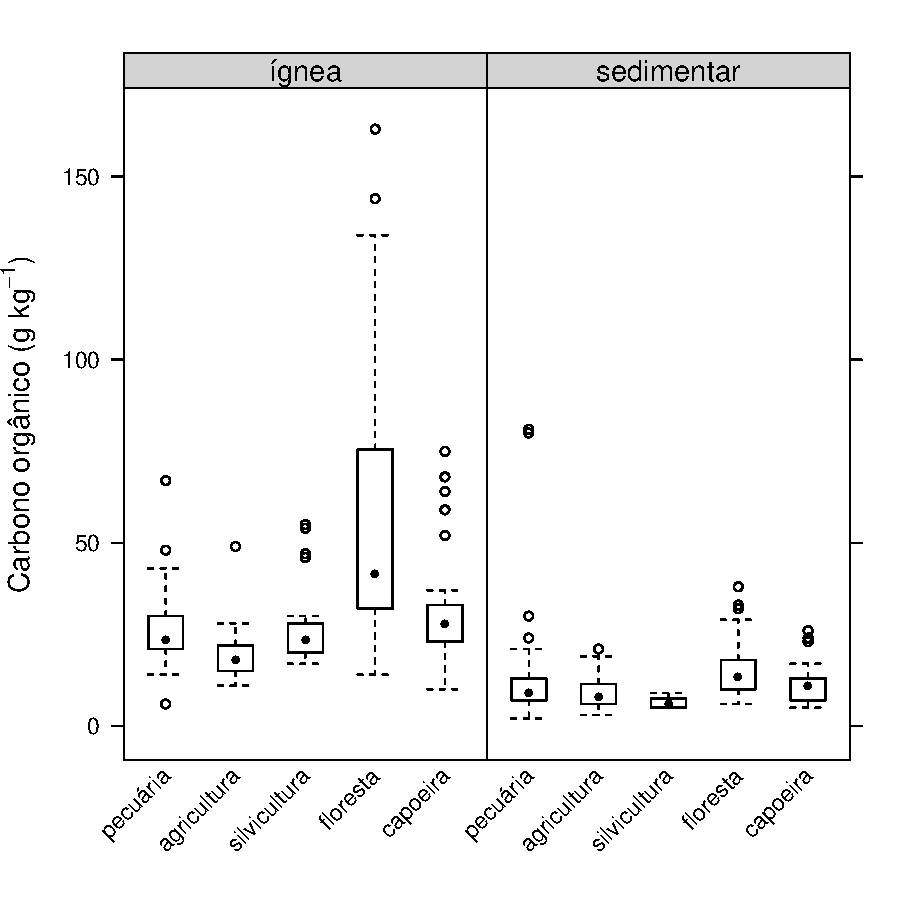
\includegraphics[width=0.60\textwidth]{fig/chap03-orca-land-parent}
\caption[Carbono orgânico no solo e sua relação com o uso da terra e o material de origem do solo.]{
Distribuição do conteúdo de carbono orgânico (\si{\gram\per\kilo\gram}) na camada superficial do solo 
(\SI{\leq20}{\cm}) e sua relação com o uso da terra e vegetação (pecuária, agricultura, silvicultura, floresta 
e capoeira) e o tipo de material de origem (ígnea -- rocha ígnea, ou sedimentar -- rocha sedimentar ou 
sedimentos diversos). O conteúdo de carbono é mais elevado em solo florestal, independente do tipo de rocha 
que deu origem ao solo. Contudo, o conteúdo de carbono é notadamente maior quando o solo tem rocha ígnea como 
material originário, sugerindo uma íntima relação com o conteúdo de argila do solo 
(\autoref{fig:chap03-clay-land-parent}) e de cátions básicos liberados durante o intemperismo do material de 
origem, refletido na capacidade de troca de cátions efetiva do solo (\autoref{fig:chap03-ecec-land-parent}). A 
grande variação no conteúdo de carbono em solo florestal reflete a ocorrência de vários estágios de sucessão 
florestal.}
\label{fig:chap03-orca-land-parent}
\end{figure}

Existe consenso de que a pequena profundidade do solo na maior parte da bacia do DNOS seja devida ao material 
de origem, às condições geomorfológicas e hidrológicas, bem como aos sistemas de cultivo do solo empregados ao 
longo de inúmeras décadas. Contudo, a diversidade de fatores e a escassez de estudos torna impossível isolar a 
contribuição individual de cada fator. Por exemplo, não existe estimativa quantitativa do volume total de solo 
perdido devido à erosão em áreas de produção agrossilvopastoril. Entretanto, acredita-se que horizontes 
pedogenéticos inteiros tenham sido removidos, dando origem ao processo de retrocesso pedogenético do solo
\cite{SamuelRosaEtAl2011a}. Esse processo reflete a involução da classificação taxonômica do solo dentro de um 
determinado sistema taxonômico. A comum ocorrência do táxon Neossolo Litólico com solum de pouco menos de 
\SI{50}{\cm} em inúmeras áreas de produção agrícola é usada para corroborar essa hipótese. Isso porque o valor 
de \SI{50}{\cm} para o solum é aquele usado para distinguir os taxa Neossolo Litólico e Neossolo Regolítico no 
Sistema Brasileiro de Classificação do Solo \cite{SantosEtAl2013a}. A mesma hipótese foi levantada em outras 
regiões de topografia complexa para explicar a identificação dos taxa Cambissolo e Luvissolo onde antes 
observava-se o táxon Chernossolo \cite{StreckEtAl2008}. Essa involução da classificação taxonômica seria 
resultado da remoção do horizonte pedogenético A chernozêmico devido à erosão acelerada pelo uso agrícola 
extrativista e intenso praticado por várias décadas. Em resumo, nas áreas onde a taxa de formação do solo é 
semelhante à taxa de erosão natural, o uso agrossilvopastoril da terra sem adoção de práticas 
conservacionistas invariavelmente resultaria na degradação do solo e consequente retrocesso pedogenético 
porque a soma das taxas de erosão natural e erosão induzida seria maior do que a taxa de formação do solo.

\begin{figure}[!ht]
\centering
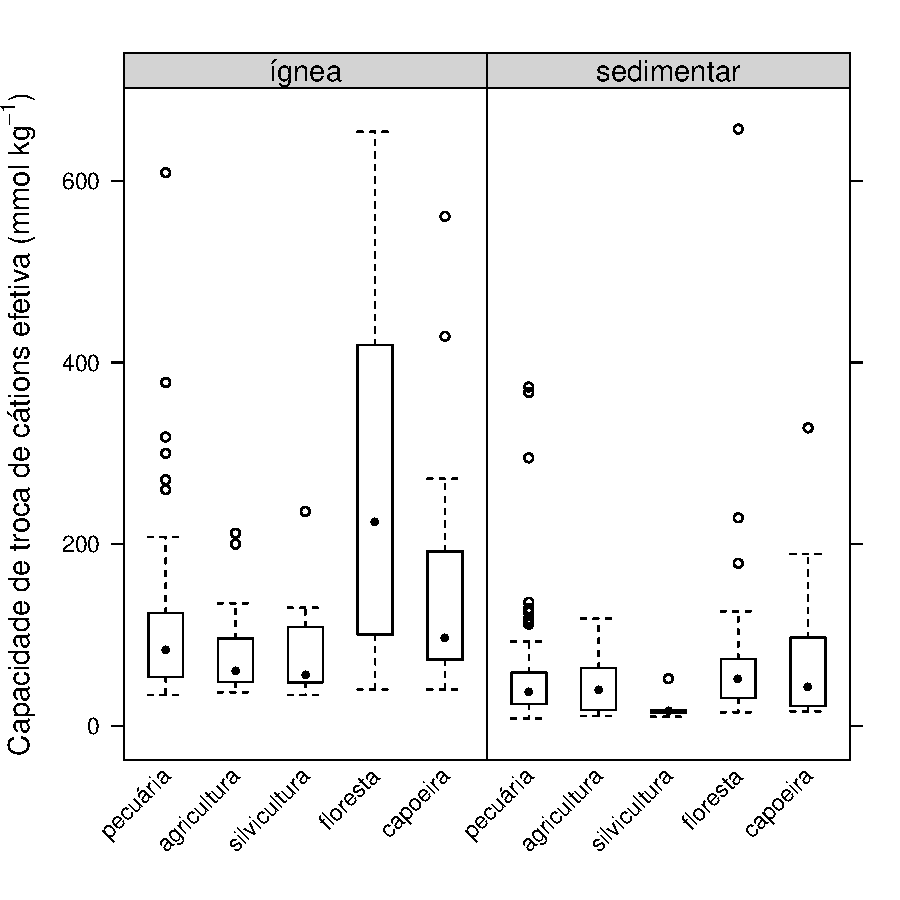
\includegraphics[width=0.60\textwidth]{fig/chap03-ecec-land-parent}
\caption[Capacidade de troca de cátions efetiva no solo e sua relação com o uso da terra e o material de 
origem do solo.]{Distribuição da capacidade de troca de cátions efetiva (\si{\milli\mole\per\kilo\gram}) na 
camada superficial do solo (\SI{\leq20}{\cm}) e sua relação com o uso da terra e vegetação (pecuária, 
agricultura, silvicultura, floresta e capoeira) e o tipo de material de origem (ígnea -- rocha ígnea, ou 
sedimentar -- rocha sedimentar ou sedimentos diversos). Assim como o conteúdo de carbono orgânico do solo, a 
capacidade de troca de cátions é maior em solo florestal. Contudo, áreas em estádio recente de regeneração 
(capoeira) e pecuária também se destacam pela elevada capacidade de troca de cátions. O contrário ocorre em 
tipos de uso da terra onde ocorre significativa exportação dos cátions do solo, caso da agricultura e 
silvicultura.}
\label{fig:chap03-ecec-land-parent}
\end{figure}

As áreas com maior potencial de desenvolvimento pedogenético em profundidade possuem menor expressão 
territorial. Elas correspondem à paisagem menos declivosa do Planalto (rochas vulcânicas), algumas coxilhas 
(rochas sedimentares) e depósitos aluviais \cite{Miguel2010}. Em áreas de material de origem vulcânica, 
sobretudo basaltos-andesitos toleíticos, identifica-se o táxon Argissolo Vermelho Alítico típico, que 
caracteriza solo com horizonte superficial de textura arenosa a média, sobrejacente a um horizonte 
subsuperficial de textura média a argilosa \cite{Miguel2010}. Nas áreas do Planalto em que ocorrem 
riólitos-riodacitos granofíricos, o solo costuma apresentar menor profundidade, sendo predominantemente 
classificado como Neossolo Litólico e Cambissolo Háplico. Em pequenas manchas, o solo é classificado como 
Argissolo Vermelho-Amarelo. O menor desenvolvimento do solo em profundidade em área de riólitos-riodacitos 
granofíricos deve-se, em parte, à maior resistência dessas rochas ao intemperismo, uma vez que possui maior 
teor de sílica, sobretudo na forma de grandes de cristais de quartzo cristalizados a baixa temperatura 
(\SI{<600}{\celsius}) \cite{Pedron2007}. Contudo, a pequena profundidade do solo também resulta da degradação 
causada pelo longo uso agrossilvopastoril sem adoção de práticas conservacionistas. Até o momento é impossível 
isolar a contribuição desses dois fatores de formação sobre as características do solo.

Em áreas de material de origem sedimentar (Formação Caturrita), o solo costuma ser classificado como 
Argissolo Bruno-Acinzentado Alítico abrúptico. Trata-se de solo com horizonte superficial de textura arenosa 
que transiciona de maneira abrupta para um horizonte subsuperficial de textura argilosa \cite{Miguel2010}. 
Essa descontinuidade textural geralmente é atribuída a processos pedogenéticos, sobretudo a perda (erosão 
lateral seletiva) e translocação (argiluviação) das partículas mais finas. Contudo, devido à complexidade 
geológica e geomorfológica da área, outros fatores podem ter contribuído. O primeiro deles estaria relacionado 
às características do próprio material de origem que, por ter sido formado em ambiente fluvial durante um 
período de mudança climática no Triássico, apresenta camadas deposicionais com granulometria diferenciada 
\cite{PieriniEtAl2002}. Assim, a presença de camadas de siltitos e folhelhos poderia ter contribuído para a 
formação da descontinuidade textural. Outro fator seria uma possível contribuição dos arenitos da Formação 
Botucatu e \emph{intertrap} na Formação Serra Geral. Dado que esse material está localizado em posições 
superiores na paisagem e são bastante suscetíveis à erosão, o mesmo poderia ter contribuído para a formação do 
horizonte superficial arenoso do solo. Em ambos os casos, a descontinuidade textural seria atribuída à 
ocorrência de descontinuidade litológica, com a diferença de que no primeiro caso as litologias pertenceriam à 
mesma formação geológica.

Nas áreas deprimidas da paisagem do Planalto, formando pequenas bacias de acumulação, ou nas áreas planas ao 
longo dos cursos de água da Depressão Periférica, o solo é classificado como Planossolo Háplico Alítico típico 
\cite{Miguel2010}. Trata-se de solo com horizonte superficial de textura média sobre horizonte subsuperficial 
de textura média a argilosa, podendo ou não apresentar horizonte intermediário eluvial. Ainda mais próximo dos 
cursos de água, o solo é classificado como Neossolo Flúvico Tb Eutrófico fragmentário \cite{Miguel2010}. Como 
o seu material de origem é diverso e possui arranjamento espacial discordante, a textura do solo é variável, 
mas sempre arenosa ou média, nunca argilosa, mesmo quando presente em áreas do Planalto ou do Rebordo. Por 
fim, com expressão territorial ainda menor, o solo é classificado como Neossolo Quartzarênico Órtico típico em 
alguns patamares do Rebordo, sejam eles de origem estrutural ou da deposição de colúvios do arenito da 
Formação Botucatu.

Atualmente, o aumento da área ocupada por florestas devido ao abandono de diversas área de produção sugere que 
a bacia do DNOS esteja adentrando um período de redução da degradação do solo, exceto nas áreas de expansão 
urbana. Os processos erosivos já apresentam caráter mais pontual, onde a geomorfologia parece possuir papel 
preponderante. Segundo estimativas, apenas uma pequena fração da área apresenta perdas de solo por erosão 
laminar acima de valores toleráveis \cite{Miguel2010}. Algumas observações até mesmo indicam que essas 
estimativas estão acima da perda real de solo por erosão laminar \cite{MouraBueno2012}. Espera-se que a 
redução da degradação do solo contribua, num futuro próximo, para a construção de um entendimento mais acurado 
da relação entre o solo e os demais componentes ambientais, principalmente nas áreas florestadas recentemente 
abandonadas.
